\documentclass[12pt,a4paper]{report}

% Packages
\usepackage[utf8]{inputenc}
\usepackage[T1]{fontenc}
\usepackage{amsmath}
\usepackage{amssymb}
\usepackage[lining]{ebgaramond}
\usepackage[cmintegrals,cmbraces]{newtxmath}
\usepackage{microtype}
\usepackage{geometry}
\usepackage{tabularx}
\usepackage{graphicx}
\usepackage{longtable}
\usepackage{booktabs}
\usepackage{array}
\usepackage{listings}
\usepackage{xcolor}
\usepackage{hyperref}
\usepackage{pdflscape}
\usepackage{float}
\usepackage{enumitem}
\usepackage{makecell}
\usepackage{siunitx}
\graphicspath{{./}}

% Page layout
\geometry{
    left=1.8cm,
    right=1.8cm,
    top=2.2cm,
    bottom=2.2cm
}

% Color definitions
\definecolor{crimson}{RGB}{153, 0, 0}
\definecolor{darkblue}{RGB}{0, 0, 153}

% Hyperlink settings
\hypersetup{
    colorlinks=true,
    linkcolor=crimson,
    urlcolor=crimson,
    citecolor=crimson
}

% Allow line breaks at slashes to prevent overfull hbox
\tolerance=2000
\emergencystretch=2em

% Chapter/section title formatting
\usepackage{titlesec}
\titleformat{\chapter}{\normalfont\huge\bfseries}{}{0pt}{}[\vspace{0.3em}]
\titlespacing*{\chapter}{0pt}{0pt}{14pt}
\titleformat{\section}{\normalfont\Large\bfseries}{\thesection}{1em}{}
\titleformat{\subsection}{\normalfont\large\bfseries}{\thesubsection}{1em}{}

\setlength{\parindent}{0pt}

\begin{document}

\pagestyle{plain}

% ─────────────────────────────────────────────
%  Cover Page
% ─────────────────────────────────────────────
\begin{titlepage}
\centering
\vspace*{3cm}

{\fontsize{28}{34}\selectfont\bfseries DSP in VLSI\par}
\vspace{0.6em}
{\fontsize{20}{26}\selectfont\bfseries Homework 4\par}
\vspace{0.4em}
{\fontsize{16}{22}\selectfont\bfseries Coordinate Rotation Digital Computer (CORDIC)\par}

\vspace{1.5cm}
\textcolor{crimson}{\rule{0.6\linewidth}{1.2pt}}
\vspace{1.5cm}

{\large\bfseries Student ID}\par
\vspace{0.4em}
{\large M11407439}\par

\vspace{0.8em}

{\large\bfseries Name}\par
\vspace{0.4em}
{\large MING-HONG, LIN}\par

\vspace{2cm}

{\large\bfseries Development Environment}\par
\vspace{0.8em}
\begin{tabular}{rl}
    \textbf{HDL}              & SystemVerilog \\[4pt]
    \textbf{Simulation Tools} & Synopsys VCS and Verdi \\[4pt]
    \textbf{Synthesis Tool}   & Synopsys DC Compiler \\[4pt]
    \textbf{Process}          & TSMC 16nm (ADFP) \\[4pt]
    \textbf{Verification}     & Python \\
\end{tabular}

\vfill

\textcolor{crimson}{\rule{0.6\linewidth}{0.6pt}}\par
\vspace{0.5em}
{\small Due Date: 2026/04/15}

\end{titlepage}

% ─────────────────────────────────────────────
%  Table of Contents
% ─────────────────────────────────────────────
\tableofcontents
\newpage

% ─────────────────────────────────────────────
\chapter{Step 1 — Realize CORDIC properties}
% ─────────────────────────────────────────────
\section{Result 1 - CORDIC scaling factor}

\hrule
\vspace{0.2cm}
Please draw the figure showing $S(N)$ \textit{versus} $N$ for $N = 1\ldots 30$. (5\%)
\vspace{0.2cm}
\hrule
\vspace{0.2cm}

% -------------------------
% USER WILL FILL IN HERE
% -------------------------
\begin{figure}[H]
    \centering
    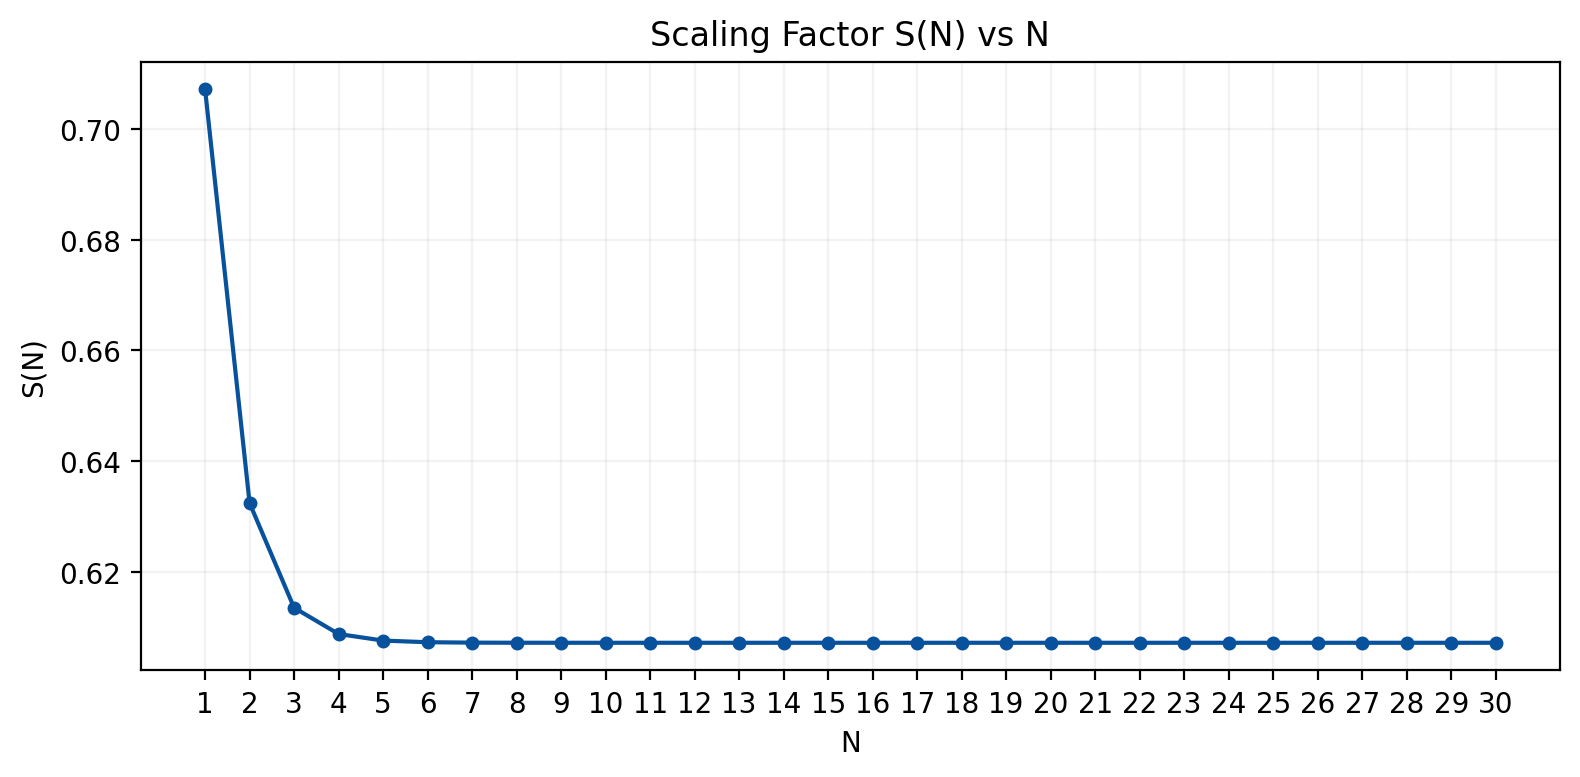
\includegraphics[width=\linewidth]{image0.png}
    \caption{Scaling Factor $S(N)$ versus Number of Micro-Rotations $N$ for $N = 1\ldots 30$}
    \label{fig:placeholder}
\end{figure}


\newpage

% ─────────────────────────────────────────────
\chapter{Step 2 — Determine the word-length of fixed-point representation}
% ─────────────────────────────────────────────
\section{Result 2 - Word-length setting}

\hrule
\vspace{0.2cm}
Draw the figure of average absolute error versus fractional wordlength (10\%) to show how you determine the setting of word-length of the fractional part. Write down the integer word-length of $X(i)$ and $Y(i)$ that you use all the stages. Please explain it. (5\%)
\vspace{0.2cm}
\hrule
\vspace{0.5cm}

From Figure 1.1, we can observe that after more than 4 micro-rotation iterations, S(N) saturates at approximately 0.6, implying that the scaling factor K(N) accumulated through micro-rotations converges to roughly 1.6. Therefore, in addition to the minimum of 9 fractional bits required as indicated by Figure 2.1, one integer bit and one sign bit must also be included, \textbf{bringing the total fixed-point representation to 11 bits.}

\begin{figure}[H]
    \centering
    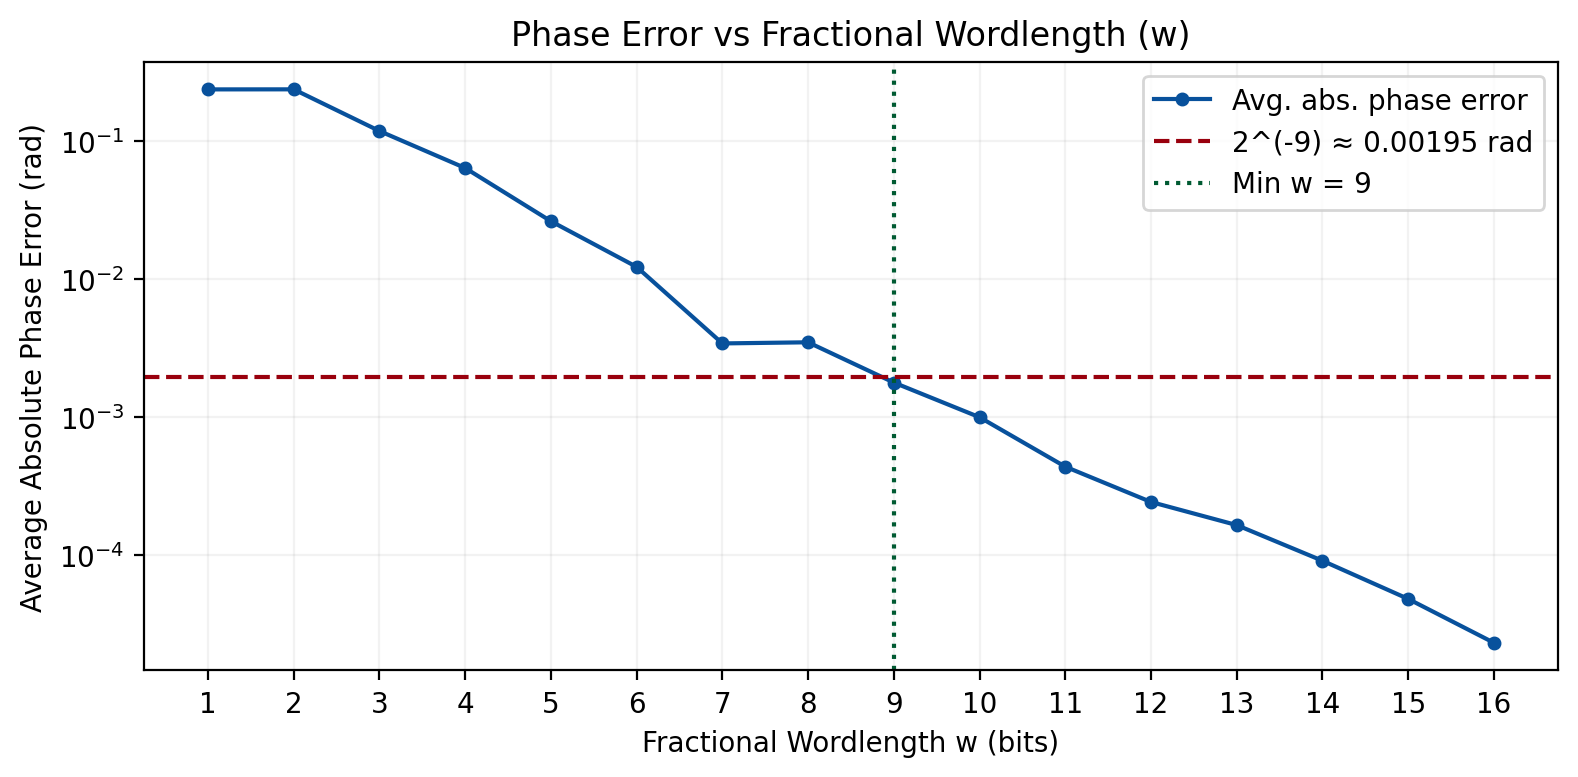
\includegraphics[width=\linewidth]{image1.png}
    \caption{Average Absolute Phase Error versus Fractional Wordlength $w$}
    \label{fig:placeholder}
\end{figure}

\newpage

% ─────────────────────────────────────────────
\chapter{Step 3 — Determine the number of micro rotations for arctangent function}
% ─────────────────────────────────────────────
\section{Result 3 - Micro-rotations and elementary angles}

\hrule
\vspace{0.2cm}
Please draw a figure to denote the average phase errors of 10 quantized input pairs $(X, Y)$ versus different numbers of micro-rotations $S$ (10\%) and draw a figure to show the resulted phase errors of 10 quantized input pairs versus the word-length of quantized elementary angles (10\%). Explain your selection to satisfy the averaged error criterion of $2^{-9}$ radian. Also list a table of the elementary angles (both in floating-point representation and binary fixed-point representation). (5\%)
\vspace{0.2cm}
\hrule
\vspace{0.2cm}

\begin{figure}[H]
    \centering
    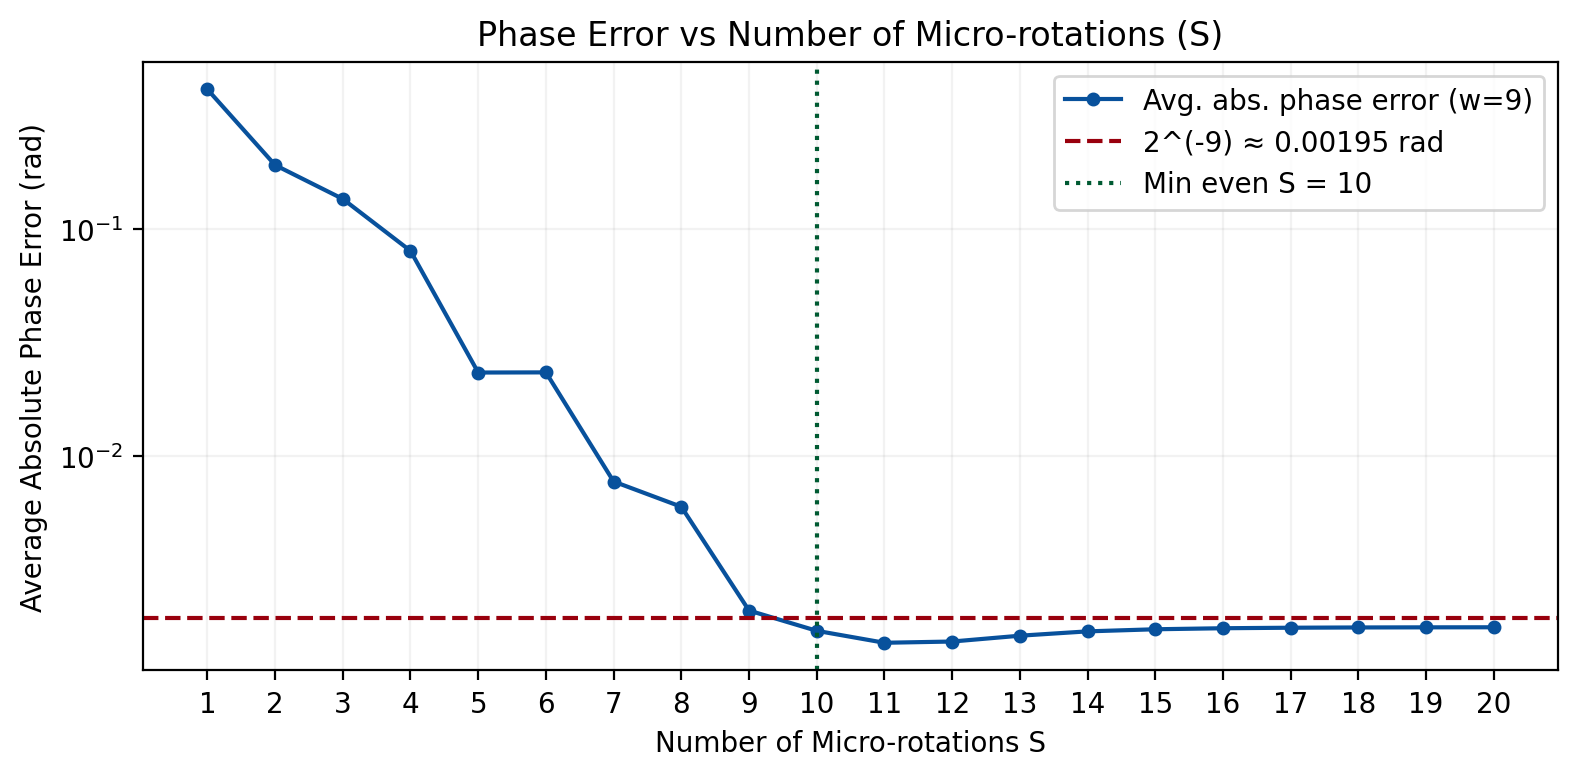
\includegraphics[width=1\linewidth]{image2.png}
    \caption{Average Phase Error of 10 Quantized Input Pairs versus Number of Micro-Rotations $S$}
    \label{fig:placeholder}
\end{figure}

\newpage

From Figure 3.2, the minimum word length satisfying the error requirement is 8 bits. However, as will be shown in the subsequent analysis, adopting 8-bit representation for the elementary angles implies that the phase accumulator and the initialization compensation value $\pi$ are also represented in 8 bits, which leads to excessive phase accumulation error that fails to meet the error threshold. \textbf{Therefore, a word length of 10 bits is adopted in this work.}

\begin{figure}[H]
    \centering
    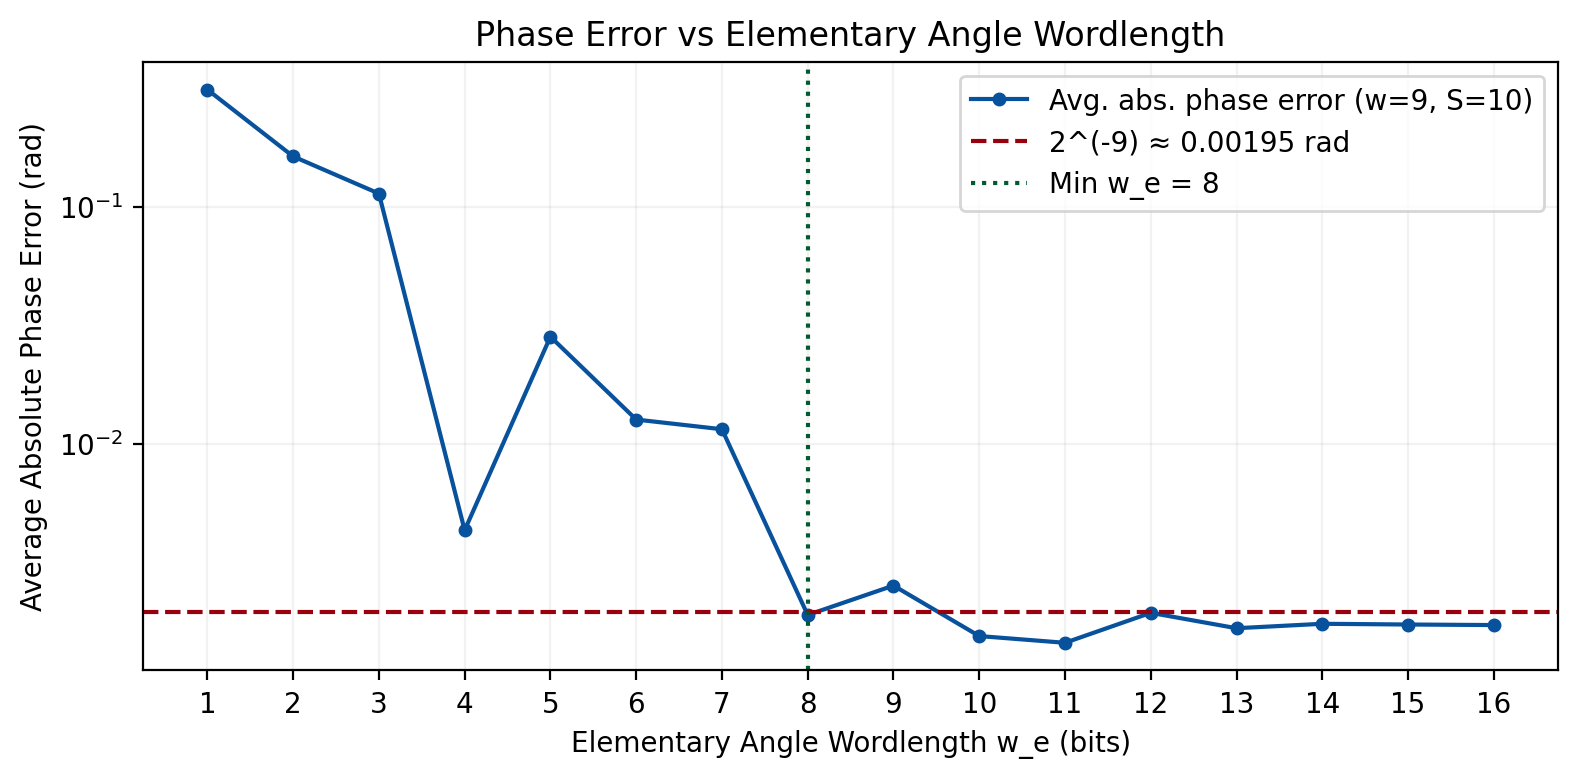
\includegraphics[width=1\linewidth]{image3.png}
    \caption{Average Phase Error of Quantized Elementary Angles}
    \label{fig:placeholder}
\end{figure}

The elementary angles are represented in a fixed-point format of 1S-2I-10F. The reason two integer bits are required is to align with the magnitude of Theta, since Theta ranges from -$\pi$ to $\pi$ as determined by the atan2 function, two integer bits are necessary to accommodate this range.

\begin{table}[H]
\centering
\small
\caption{Elementary Angle LUT}
\vspace{0.6em}
\setlength{\tabcolsep}{16pt}
\renewcommand{\arraystretch}{1.35}
\begin{tabular}{c S[table-format=1.10, group-digits=false] c}
\toprule
\textbf{i} & \textbf{{Floating-Point}} & \textbf{{Fixed-Point (Binary)}} \\
\midrule
0 & 0.7853981634 & \texttt{0\;00\;1100100100} \\
1 & 0.4636476090 & \texttt{0\;00\;0111011011} \\
2 & 0.2449786631 & \texttt{0\;00\;0011111011} \\
3 & 0.1243549945 & \texttt{0\;00\;0001111111} \\
4 & 0.0624188100 & \texttt{0\;00\;0001000000} \\
5 & 0.0312398334 & \texttt{0\;00\;0000100000} \\
6 & 0.0156237286 & \texttt{0\;00\;0000010000} \\
7 & 0.0078123411 & \texttt{0\;00\;0000001000} \\
8 & 0.0039062301 & \texttt{0\;00\;0000000100} \\
9 & 0.0019531225 & \texttt{0\;00\;0000000010} \\
\bottomrule
\end{tabular}
\end{table}

\newpage

% ─────────────────────────────────────────────
\chapter{Step 4 — Determine the number of micro rotations for magnitude function}
% ─────────────────────────────────────────────
\section{Result 4 - Number of micro-rotations for magnitude function}

\hrule
\vspace{0.2cm}
Please show how you decide the number of micro-rotations for the magnitude function with error tolerance of 0.1\%. (10\%)
\vspace{0.2cm}
\hrule
\vspace{0.4cm}

From Eq.~(11) in the homework specification, the relative error of approximating the magnitude function using $N$ micro-rotations is bounded by

\begin{equation}
\frac{|X+jY| - S(N)\,X(N)}{|X+jY|}
= 1 - \cos\!\bigl(\theta'(N)\bigr)
\end{equation}

where $\theta'(N)$ is the residual phase after $N$ micro-rotations. Since $\theta'(N)$ must be smaller than the last elementary angle $\theta_e(N-1) = \tan^{-1}(2^{-(N-1)})$, the error upper bound becomes (Eq.~12):

\begin{equation}
\text{Error} < 1 - \cos\!\bigl(\theta_e(N-1)\bigr)
= 1 - \frac{1}{\sqrt{1 + 2^{-2(N-1)}}}
\end{equation}

Imposing the 0.1\% ($= 10^{-3}$) tolerance and solving directly for $N$:

\begin{align}
1 - \frac{1}{\sqrt{1 + 2^{-2(N-1)}}} &< 10^{-3} \notag \\
\frac{1}{\sqrt{1 + 2^{-2(N-1)}}} &> 1 - 10^{-3} \notag \\
1 + 2^{-2(N-1)} &< \frac{1}{(1-10^{-3})^{2}} \notag \\
2^{-2(N-1)} &< \frac{1}{(0.999)^{2}} - 1 \approx 2.003 \times 10^{-3} \notag \\
-2(N-1) &< \log_{2}\!\bigl(2.003\times10^{-3}\bigr) \approx -8.96 \notag \\
N - 1 &> 4.48 \notag \\
N &> 5.48
\end{align}

Since $N$ must be a positive integer, $\mathbf{N_{\min} = 6}$.
\textbf{Therefore, a minimum of 6 micro-rotations is required to meet the 0.1\% error tolerance for the magnitude function.}

\newpage

% ─────────────────────────────────────────────
\chapter{Step 5 — Determine the CSD of the scaling factor}
% ─────────────────────────────────────────────
\section{Result 5 - CSD representation and shift-and-add block}

\hrule
\vspace{0.2cm}
Write a program to show the setting of fractional wordlength of CSD versus error. Draw the figure. (10\%). Depict your design for the shift-and-add block according to your CSD representation. How many adders do you use? (10\%)
\vspace{0.2cm}
\hrule
\vspace{0.2cm}

\begin{figure}[H]
    \centering
    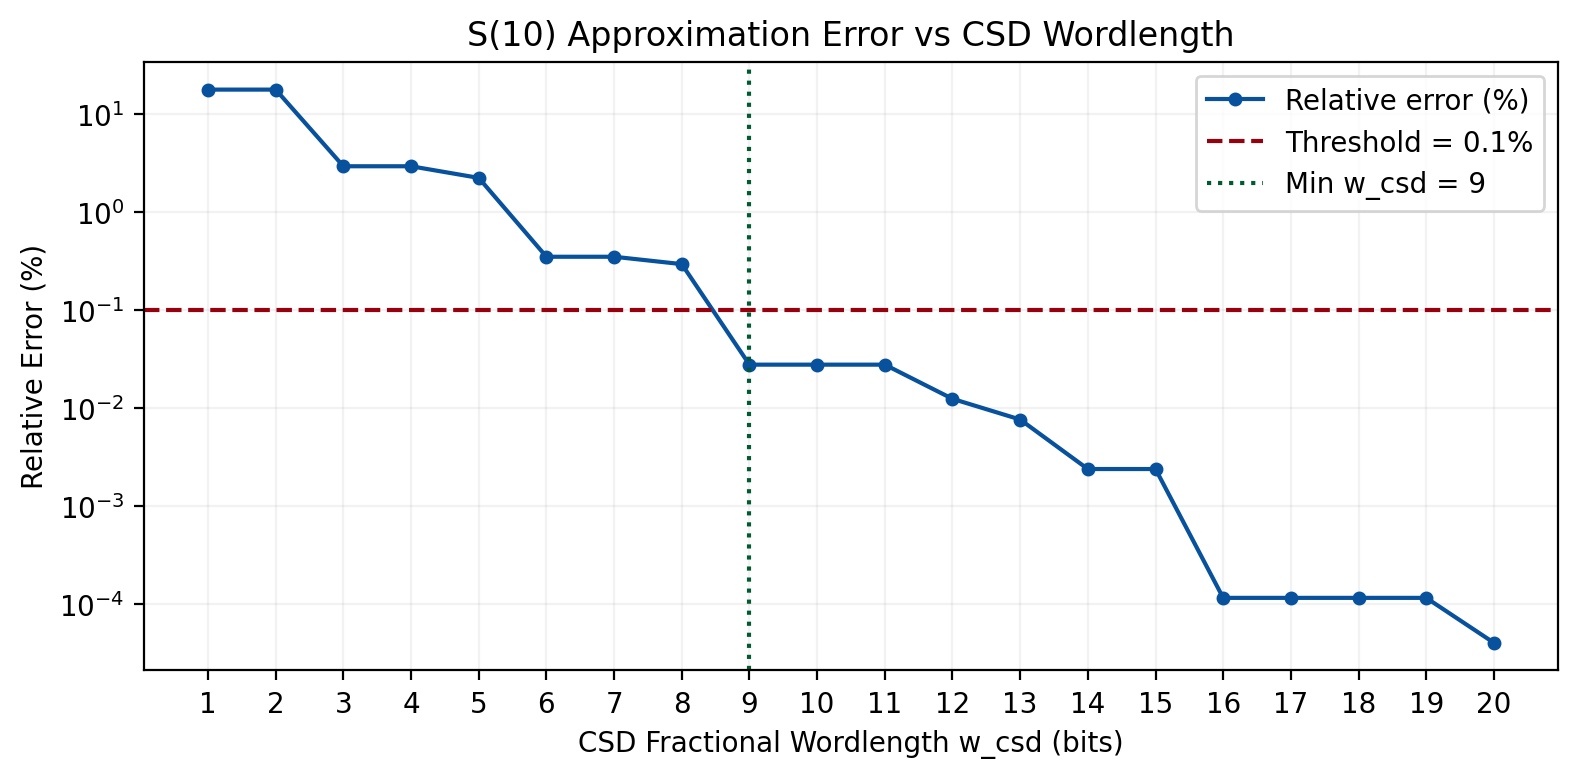
\includegraphics[width=0.8\linewidth]{image4.png}
    \caption{Scaling Factor Approximation Error versus Fractional Wordlength of CSD Representation}
    \label{fig:placeholder}
\end{figure}

To satisfy the 0.1\% error tolerance, the scaling factor $S(N)$ is converted to the CSD
sequence $(0.10100100\bar{1})_{\text{CSD}}$ with a 9-bit fractional wordlength. This corresponds to
$2^{-1} + 2^{-3} + 2^{-6} - 2^{-9}$. Since this expression contains 4 non-zero terms, the shift-and-add module 
requires exactly \textbf{3 adders}, matching the architecture in Figure 5.2.

\begin{figure}[H]
    \centering
    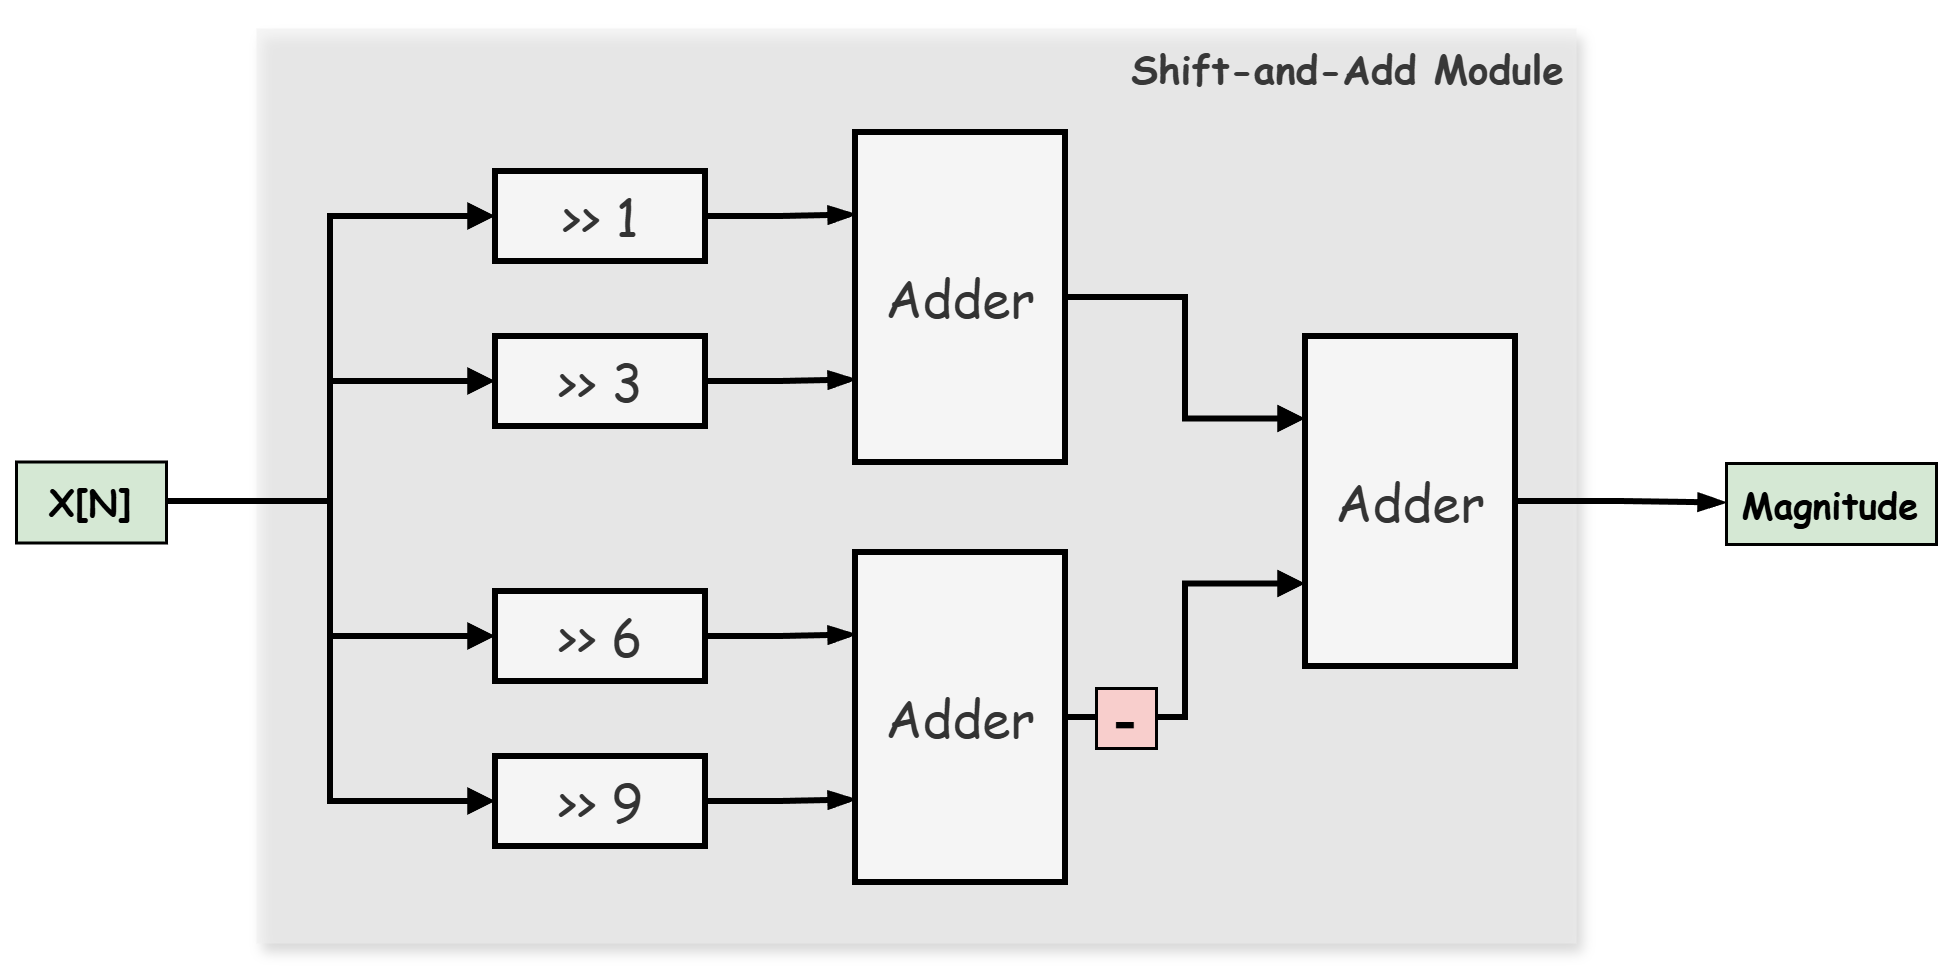
\includegraphics[width=0.8\linewidth]{CSD.png}
    \caption{Shift-and-Add Block Diagram for Scaling Factor $S(N)$ Using CSD Representation}
    \label{fig:placeholder}
\end{figure}



\newpage

% ─────────────────────────────────────────────
\chapter{Step 6 — Iterative architecture design}
% ─────────────────────────────────────────────
\section{Result 6.1 - Initial stage design}

\hrule
\vspace{0.2cm}
Depict your design of the initial stage. Mark the word-length in the block diagram. (10\%)
\vspace{0.2cm}
\hrule
\vspace{0.2cm}

\begin{figure}[H]
    \centering
    
\includegraphics[width=0.75\linewidth]{Result6.png}
    \caption{Block Diagram of the Initial Stage with Word-Length Annotations}
    \label{fig:placeholder}
\end{figure}

\newpage

\section{Result 6.2 - Iterative architecture behavior simulation}

\hrule
\vspace{0.2cm}
Implement your design with only DFFs inserted at the inputs and outputs. Show the timing diagram of behavior simulation for four inputs. (15\%) Compare the results with the arctangent function and draw the error versus index $m$ to show that your implementation meets the precision requirements of error less than $2^{-9}$. (10\%)
\vspace{0.2cm}
\hrule
\vspace{0.2cm}

\subsection*{Hardware Configuration Summary}

The following table summarizes the hardware configuration derived from the analysis above.

\begin{table}[h]
\centering
\begin{tabular}{|c|c|c|c|}
\hline
\textbf{Parameter} & \textbf{Bit-Width} & \textbf{Description} & \textbf{Error Analyzed} \\
\hline
Input $X$ and $Y$               & 1S-1I-9F & 11-bit signed fixed-point                          & \checkmark \\
Elementary Angle $\theta_e$         & 1S-2I-8F & 11-bit, matches $\theta$ range & \checkmark \\
Accumulated Angle $\theta$       & 1S-2I-8F & 11-bit, matches fraction of $\theta_e$                    & $\times$ \\
Initial Rotation Angle  $\theta_i$       & 1S-2I-8F & 11-bit, matches $\theta_e$ and $\theta$ format        & $\times$ \\
Number of Micro-Rotations        & ---      & 10 iterations                                      & \checkmark \\
Magnitude Output                 & 1S-1I-9F & Matches input format                               & $\times$ \\
\hline
\end{tabular}
\caption{Hardware Configuration Summary for CORDIC Design}
\end{table}

Note that not all parameters listed above have been individually analyzed for error. Therefore, directly applying the hardware configuration above is insufficient to guarantee that the design meets the required error constraints, specifically, that the phase error of $\theta$ remains below $2^{-9}$ radians and that the magnitude error stays within 0.1\%.

\vspace{0.5cm}

To address this, all relevant hardware parameters were incorporated into a Python simulation to determine the minimum configuration that satisfies both error thresholds. The resulting parameters are summarized in the table below.

\begin{table}[h]
\centering
\begin{tabular}{|c|c|c|}
\hline
\textbf{Parameter} & \textbf{Bit-Width} & \textbf{Description} \\
\hline
Input $X$ and $Y$          & 1S-1I-12F & 14-bit signed fixed-point \\
Elementary Angle            & 1S-2I-10F & 13-bit, extended integer bits to cover angle range \\
Accumulated Angle $\theta$  & 1S-2I-10F & Matches elementary angle format \\
Initial Rotation Angle      & 1S-2I-10F & Matches elementary angle and $\theta$ format \\
Number of Micro-Rotations   & ---       & 12 iterations \\
Magnitude Output            & 1S-1I-12F & Matches input format \\
\hline
\end{tabular}
\caption{Minimum Hardware Configuration to Meet Error Constraints}
\end{table}

Therefore, in the following implementation, I will adopt the parameters from Table 6.2 rather 
than Table 6.1 to ensure \textbf{compliance with the error threshold}.

\newpage

\begin{figure}[h]
    \centering
    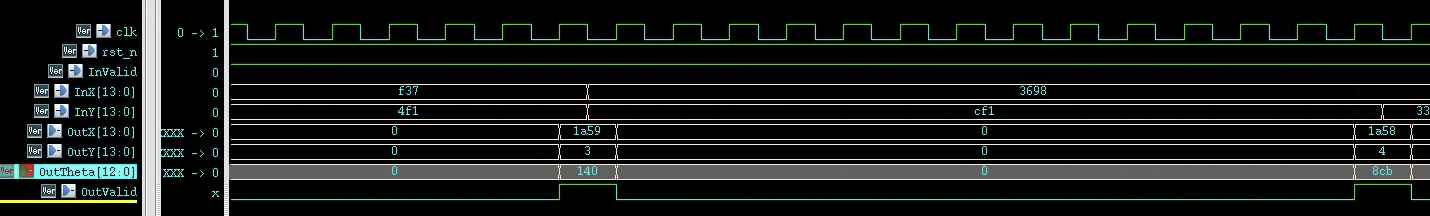
\includegraphics[width=\linewidth]{image.png}
    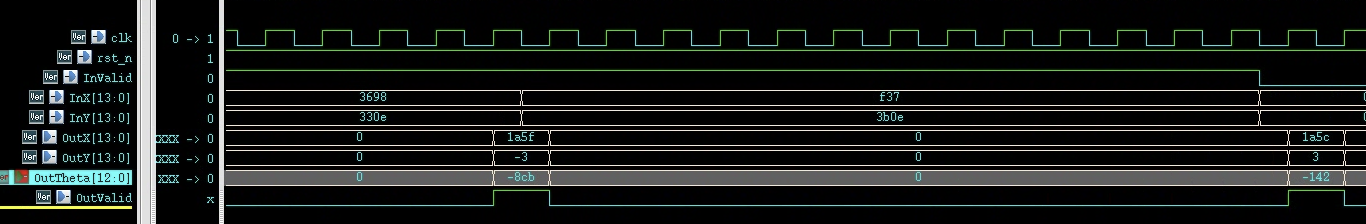
\includegraphics[width=\linewidth]{image5.png}
    \caption{Behavior Simulation Timing Diagram of Iterative CORDIC Architecture (Four Inputs)}
    \label{fig:placeholder}
\end{figure}

\begin{figure}[h]
    \centering
    \includegraphics[width=0.85\linewidth]{4output.png}
    \caption{Phase Error versus Input Index $m$ --- Iterative CORDIC Architecture}
    \label{fig:placeholder}
\end{figure}


% ─────────────────────────────────────────────
\chapter{Step 7 — Unfolding architecture design}
% ─────────────────────────────────────────────
\section{Result 7 - Unfolding architecture}

\hrule
\vspace{0.2cm}
Draw the block diagram of your $\frac{S}{2}$-unfolding architecture. (10\%). Show the timing diagram of behavior and post-synthesis simulation with correct setting of clock period and 10 inputs. (30\%) Verified the error between the post-synthesis results and the floating-point arctangent results. Draw the error versus index $m$. (10\%)
\vspace{0.2cm}
\hrule
\vspace{0.2cm}
\begin{figure}[h]
    \centering
    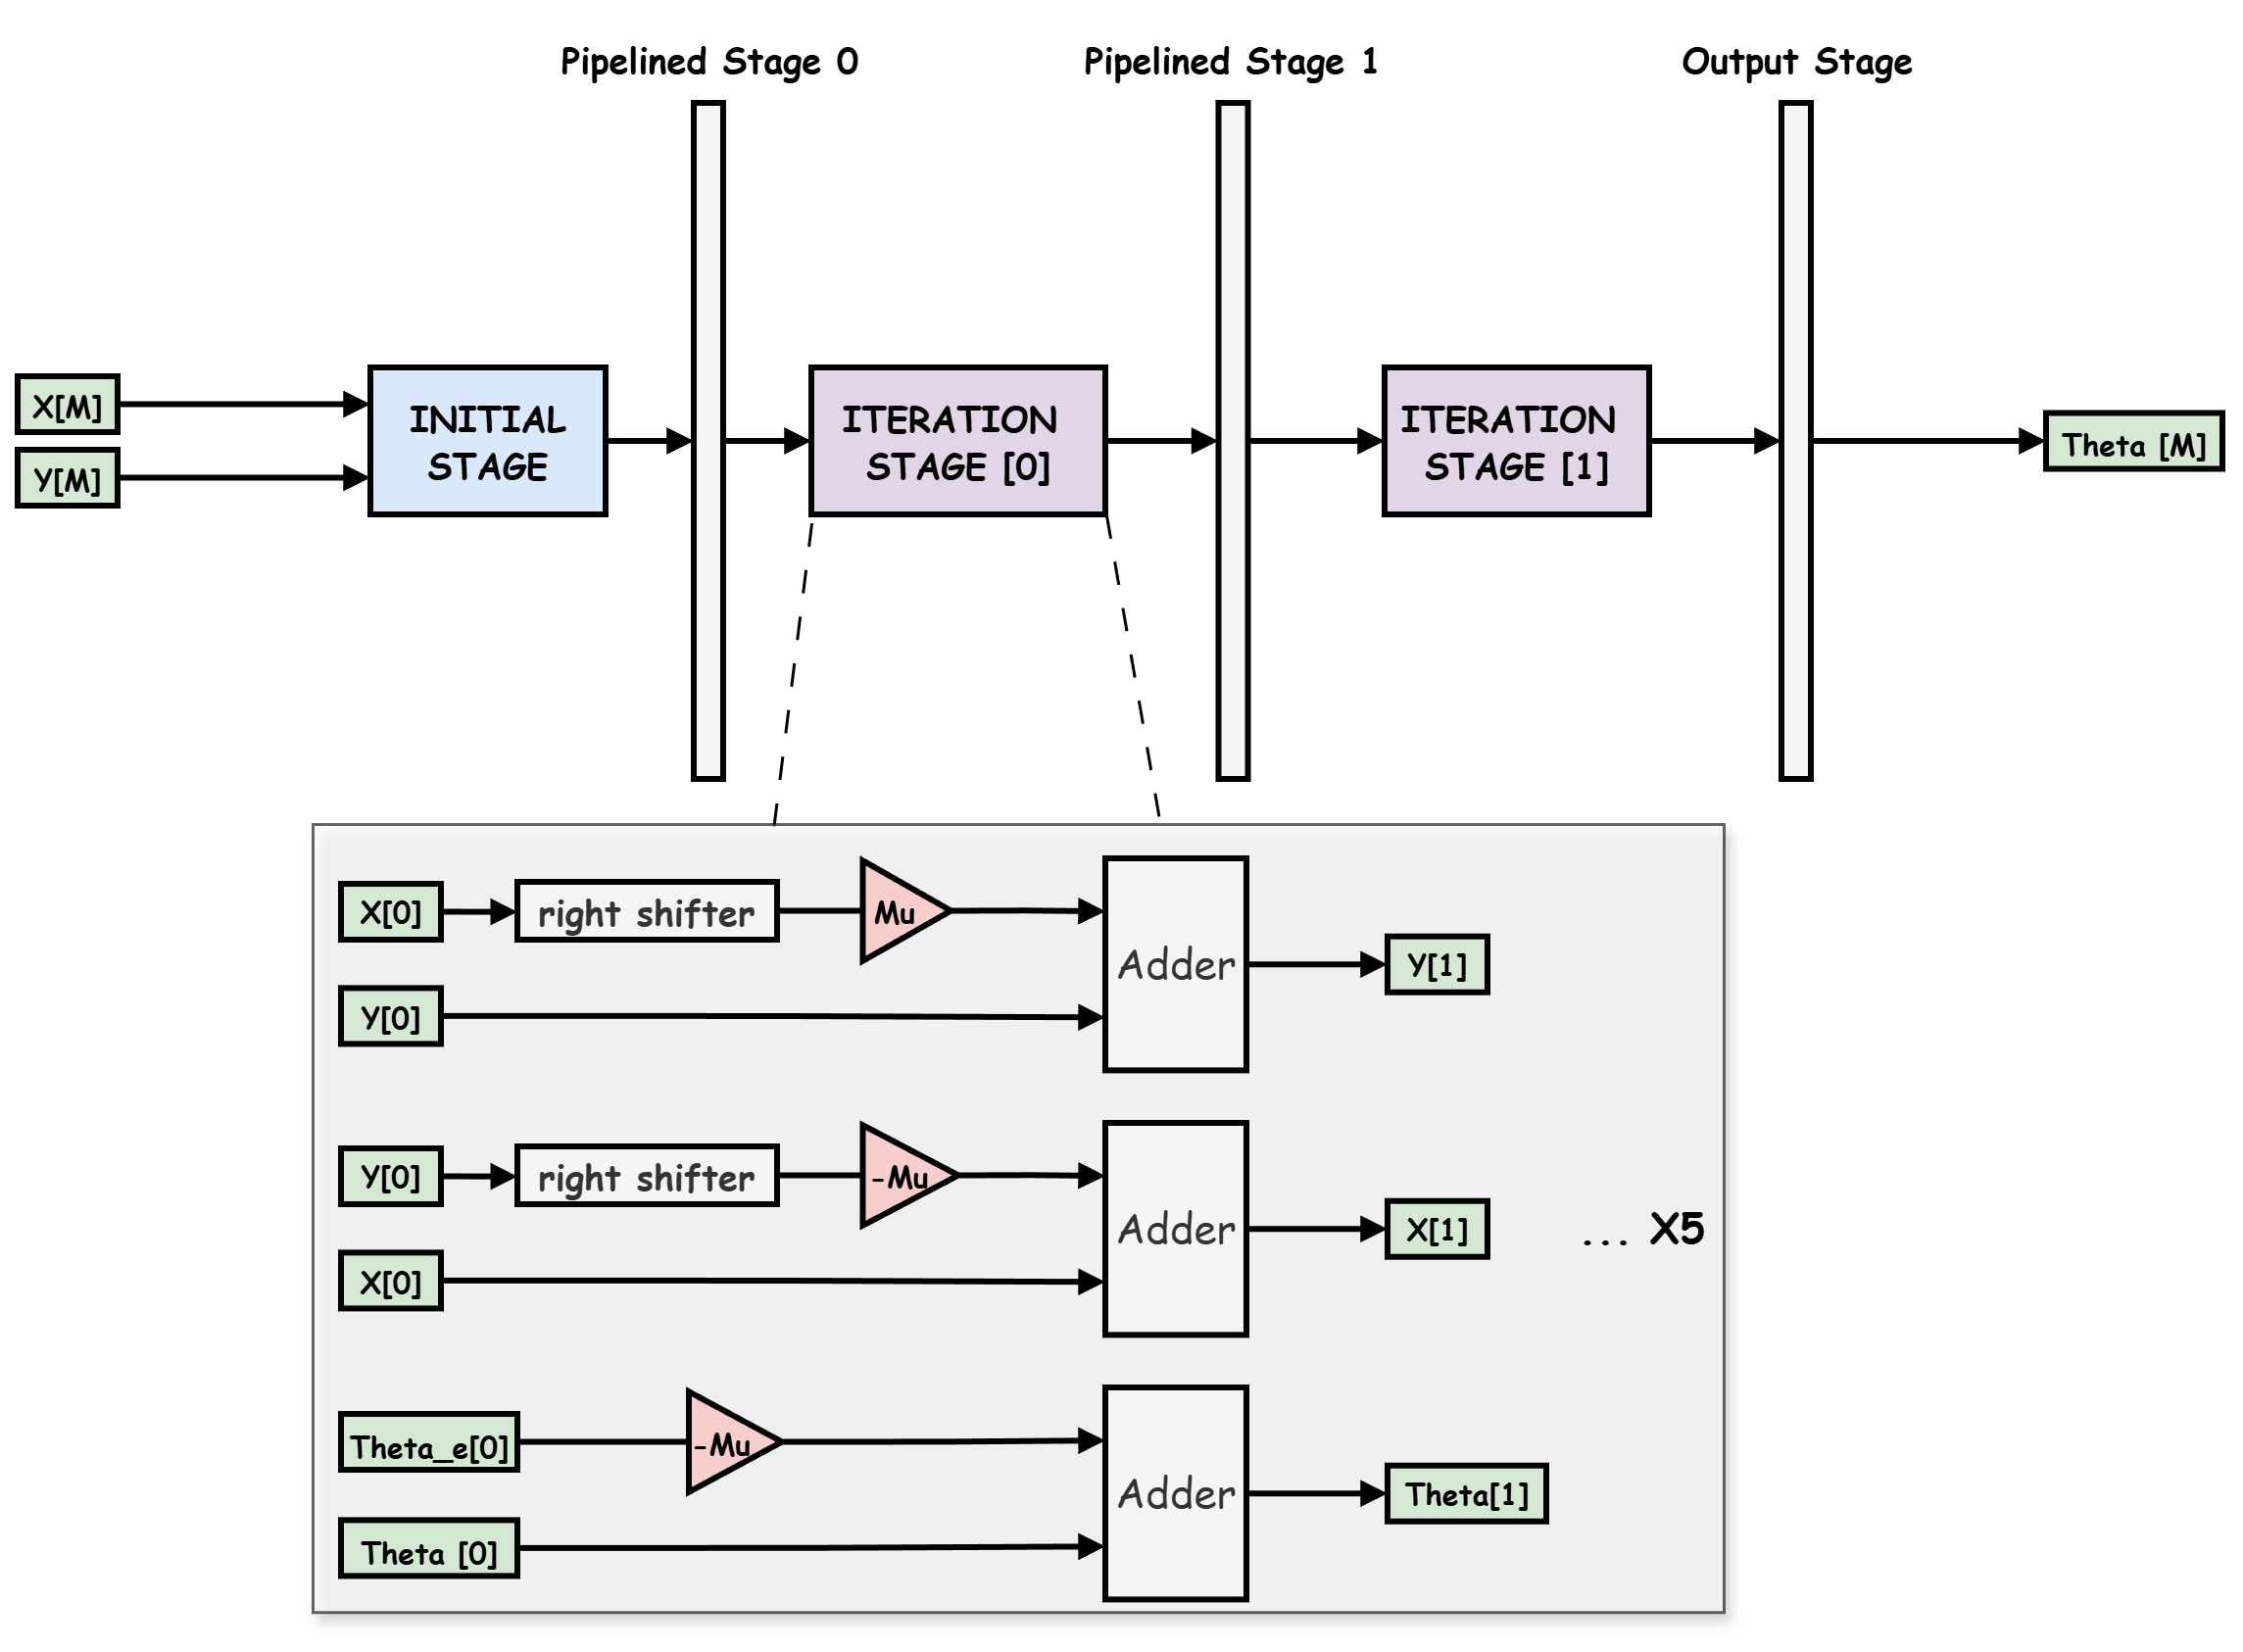
\includegraphics[width=0.75\linewidth]{Unfolding.png}
    \caption{Block Diagram of the $\frac{S}{2}$-Unfolding CORDIC Architecture}
    \label{fig:placeholder}
\end{figure}

\begin{figure}[h]
    \centering
    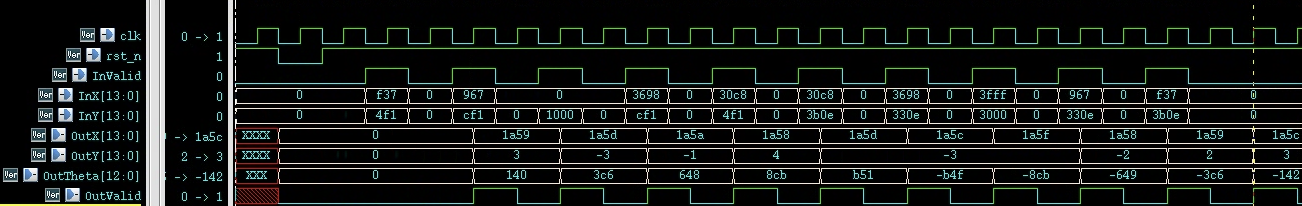
\includegraphics[width=\linewidth]{image7.png}
    \caption{Behavior Simulation Timing Diagram of Unfolding CORDIC Architecture (10 Inputs)}
    \label{fig:placeholder}
\end{figure}

\newpage

\begin{figure}[h]
    \centering
    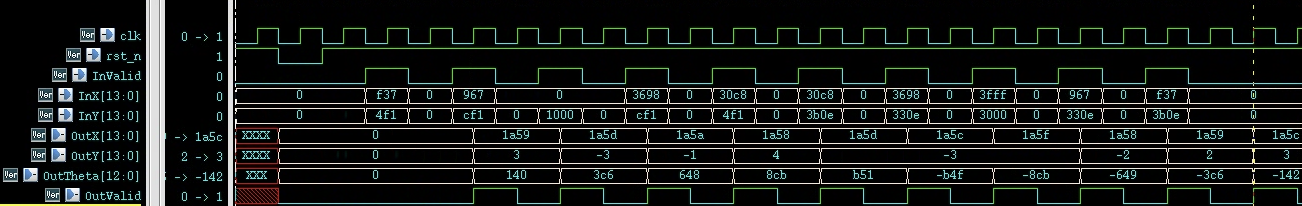
\includegraphics[width=\linewidth]{image7.png}
    \caption{Post-Synthesis Simulation Timing Diagram of Unfolding CORDIC Architecture (10 Inputs)}
    \label{fig:placeholder}
\end{figure}

\begin{figure}[H]
    \centering
    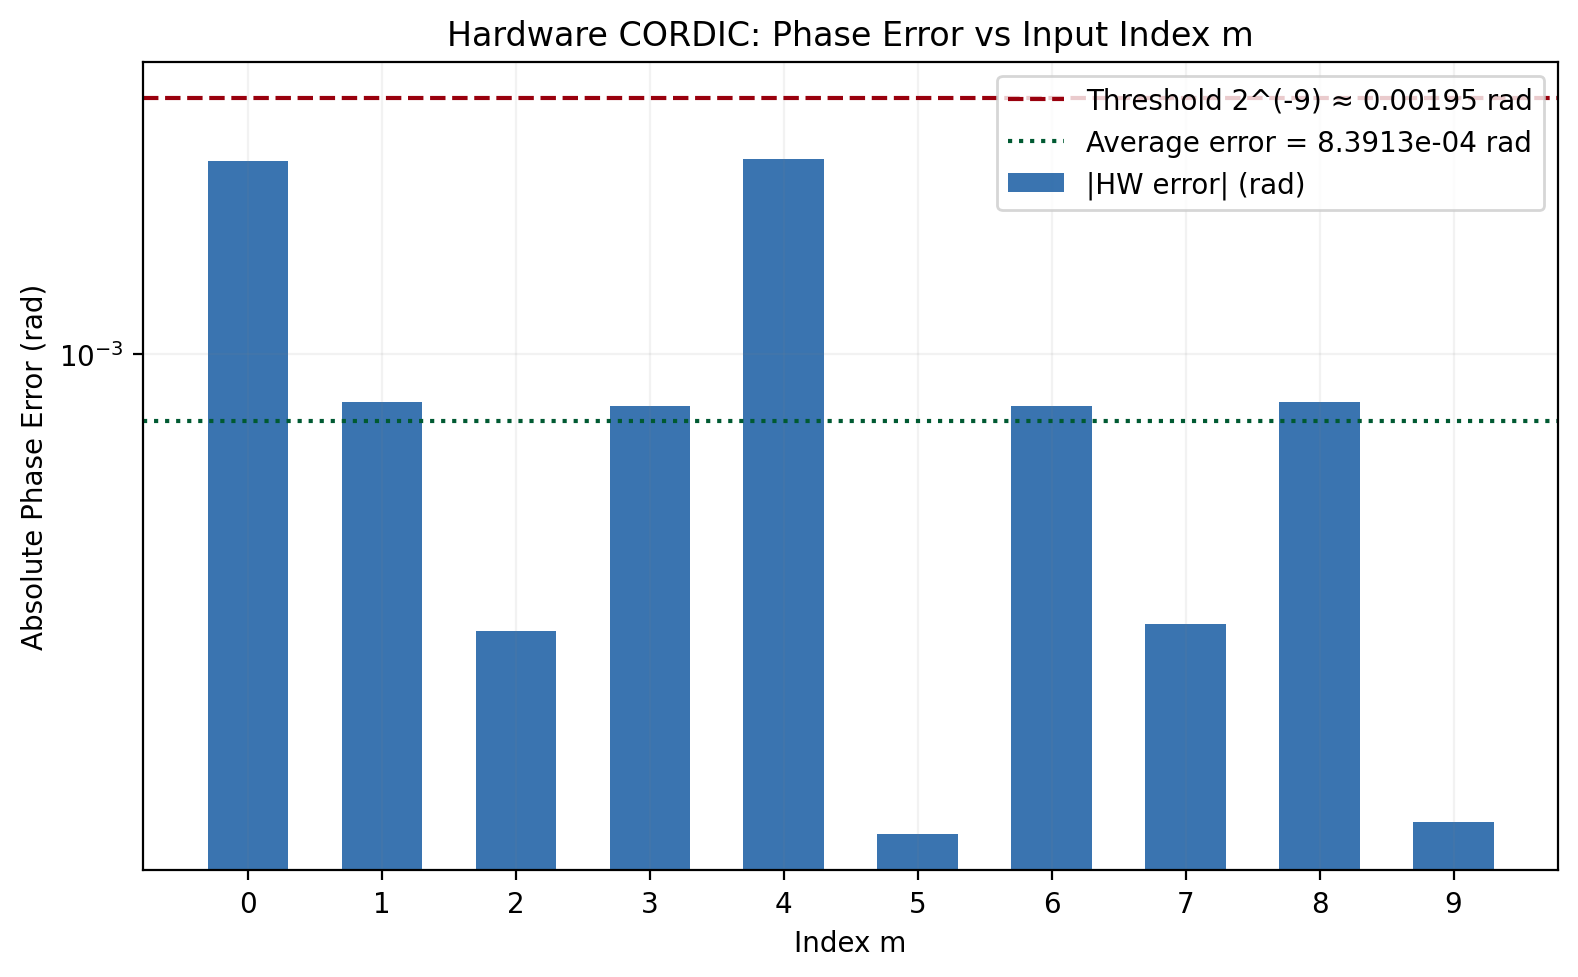
\includegraphics[width=0.85\linewidth]{image6.png}
    \caption{Phase Error versus Input Index $m$ --- Unfolding Architecture (Post-Synthesis)}
    \label{fig:placeholder}
\end{figure}

\newpage

% ─────────────────────────────────────────────
\chapter{Step 8 — Check area}
% ─────────────────────────────────────────────
\section{Result 8 - Area comparison}

\hrule
\vspace{0.2cm}
Report and compare the area before and after unfolding. (10\%)
\vspace{0.2cm}
\hrule
\vspace{0.2cm}

\begin{table}[H]
\centering
\caption{Area Comparison Before and After Unfolding}
\vspace{0.6em}
\setlength{\tabcolsep}{16pt}
\renewcommand{\arraystretch}{1.35}
\begin{tabular}{lcc}
\toprule
\textbf{Architecture} & \textbf{Clock Frequency} & \textbf{Total Cell Area (\si{\micro\metre\squared})} \\
\midrule
Folding (Iterative)       & \SI{200}{MHz} & 284.24 \\
Unfolding + Pipeline      & \SI{200}{MHz} & 763.91 \\
\midrule
\textbf{Area Overhead}    & ---           & $\mathbf{\times 2.69}$ \\
\bottomrule
\end{tabular}
\end{table}

The unfolding architecture achieves the same clock frequency of \SI{200}{MHz} but increases the total cell area by approximately $2.69\times$ compared to the folding (iterative) design. This overhead is expected, as unfolding replicates the datapath to process multiple samples per cycle, trading area for higher throughput.

\newpage

% ─────────────────────────────────────────────
\chapter{Step 9 — Hardware architecture design}
% ─────────────────────────────────────────────
\section{Result 9 - Architecture for magnitude function}

\hrule
\vspace{0.2cm}
Draw the shift-and-add module for the scaling factor (5\%). Connect the shift-and-add module to your micro-rotation module, and calculate the magnitude function. Show the timing diagram of behavior simulation and post-synthesis simulation with proper setting of clock period. (15\%). Verified the error between the post-synthesis results and the floating-point arctangent results. Draw the error versus index $m$. (10\%)
\vspace{0.2cm}
\hrule
\vspace{0.2cm}

\begin{figure}[H]
    \centering
    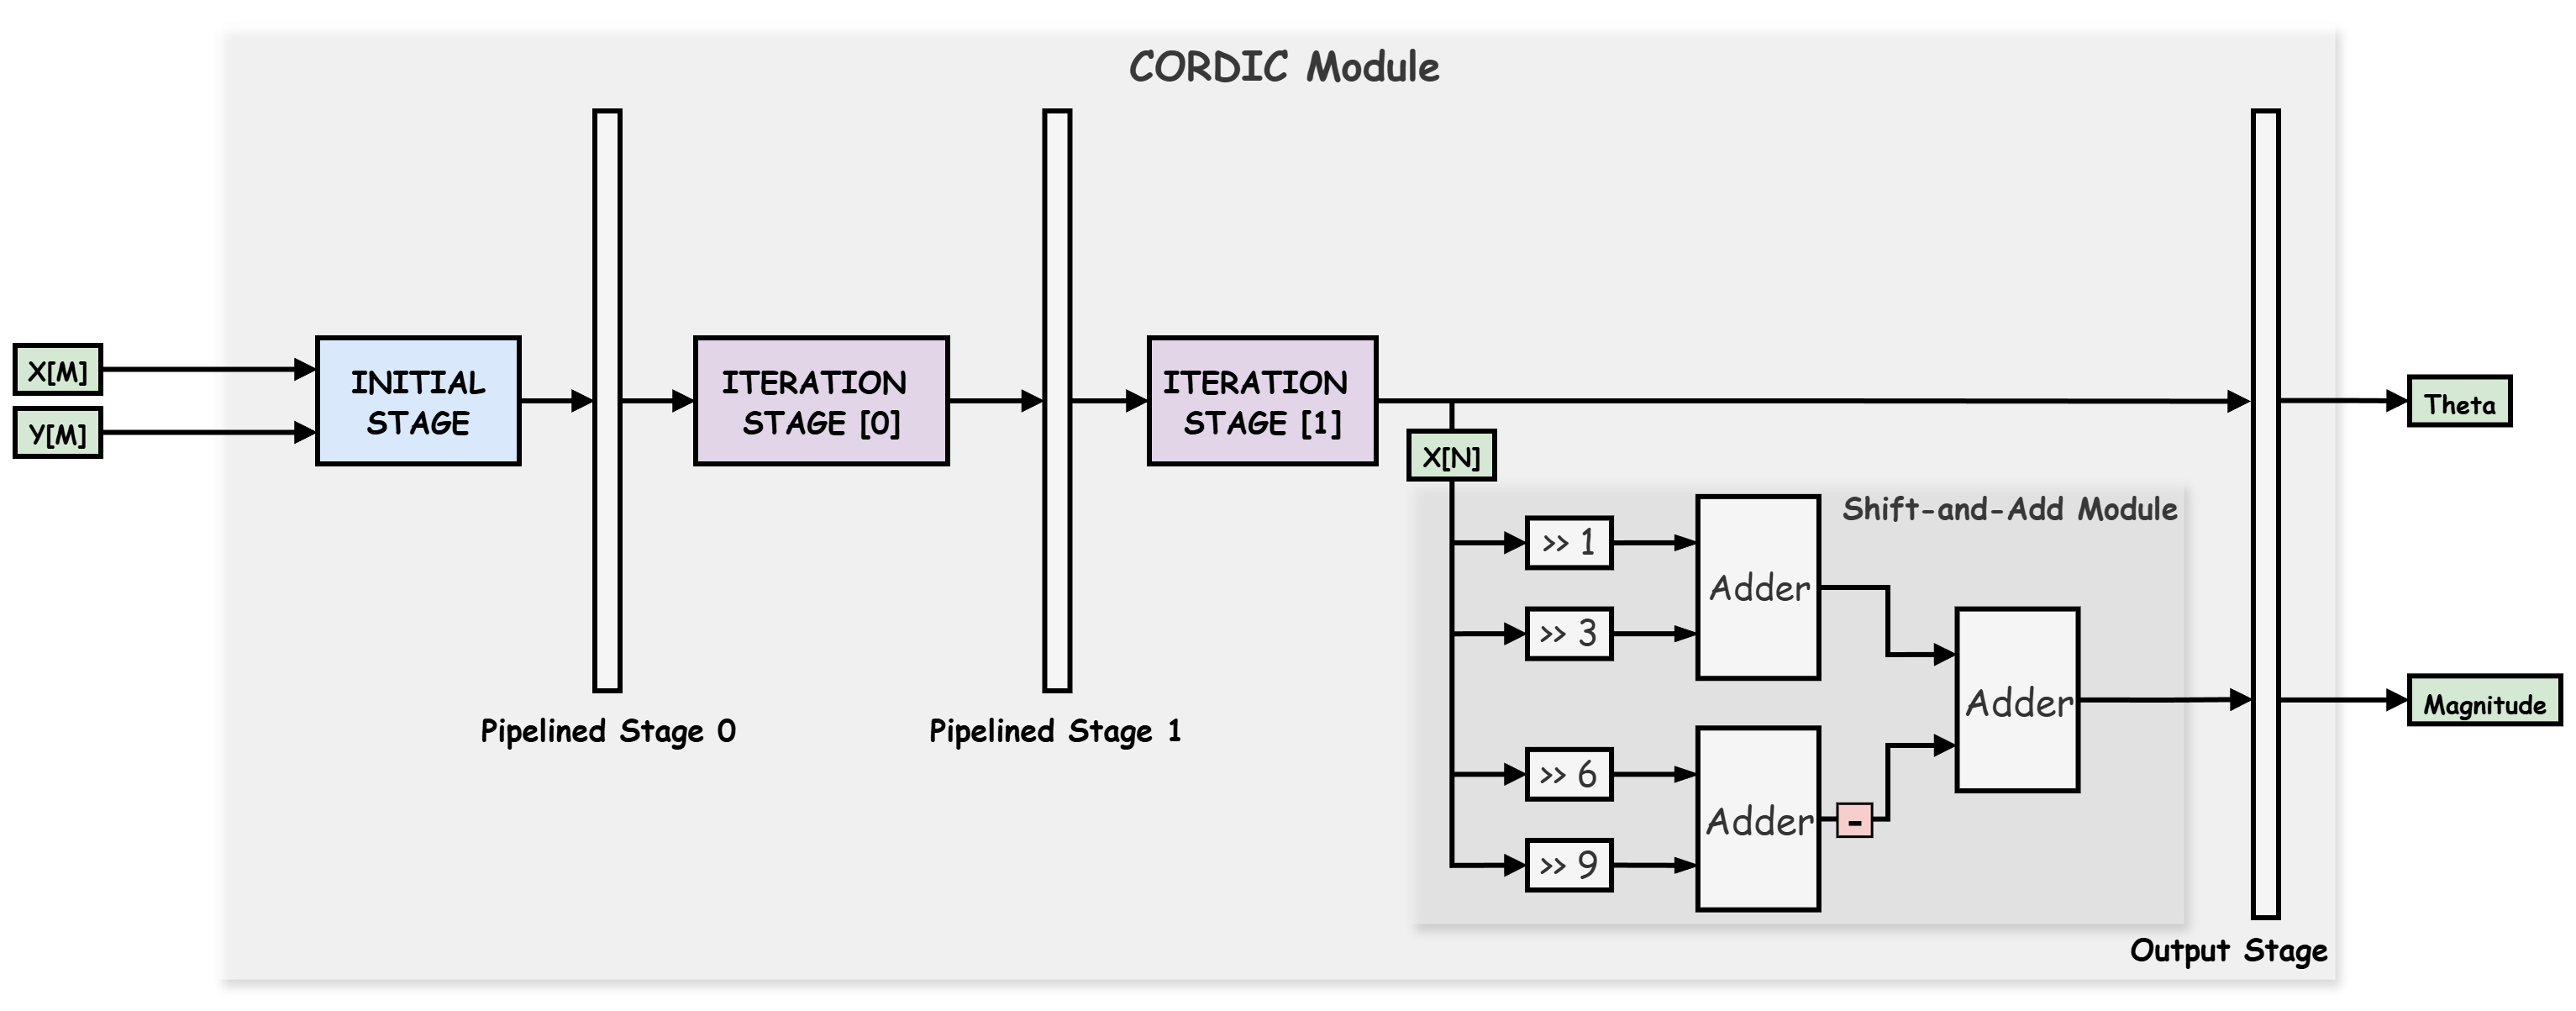
\includegraphics[width=1\linewidth]{CORDIC.png}
    \caption{Complete CORDIC Architecture Block Diagram Including Initial Stage and Scaling Stage}
    \label{fig:cordic_block}
\end{figure}

\begin{table}[H]
\centering
\caption{Synthesis Timing Constraint Summary (Clock Period = \SI{1.0}{ns}, \SI{1}{GHz})}
\vspace{0.6em}
\setlength{\tabcolsep}{14pt}
\renewcommand{\arraystretch}{1.35}
\begin{tabular}{lcc}
\toprule
\textbf{Constraint} & \textbf{Value} & \textbf{Remark} \\
\midrule
Clock Period            & \SI{1.0}{ns}   & \SI{1}{GHz} target frequency \\
Clock Latency           & \SI{0.5}{ns}   & \texttt{set\_clock\_latency} \\
Setup Uncertainty       & \SI{0.1}{ns}   & \texttt{set\_clock\_uncertainty -setup} \\
Hold Uncertainty        & \SI{0.005}{ns} & \texttt{set\_clock\_uncertainty -hold} \\
Input Delay             & \SI{0.5}{ns}   & 50\% of clock period \\
Output Delay            & \SI{0.5}{ns}   & 50\% of clock period \\
\midrule
Effective Setup Budget  & \SI{0.9}{ns}   & Period $-$ Setup Uncertainty \\
\bottomrule
\end{tabular}
\end{table}

\newpage

\begin{figure}[H]
    \centering
    \includegraphics[width=1\linewidth]{Final-Sim.png}
    \caption{Behavior Simulation --- Final CORDIC with Magnitude Output}
    \label{fig:final_sim}
\end{figure}

\begin{figure}[H]
    \centering
    \includegraphics[width=1\linewidth]{Final-Syn.png}
    \caption{Gate-Level (Post-Synthesis) Simulation --- Final CORDIC with Magnitude Output}
    \label{fig:final_syn}
\end{figure}

\begin{figure}[H]
    \centering
    \includegraphics[width=0.85\linewidth]{output.png}
    \caption{MagnitudeError versus Input Index $m$ --- Final CORDIC with Magnitude Output (Post-Synthesis)}
    \label{fig:placeholder}
\end{figure}

\end{document}